\documentclass[12pt,a4paper]{article}
\usepackage[utf8]{inputenc}
\usepackage[english]{babel}
\usepackage{amsmath}
\usepackage{amsfonts}
\usepackage{amssymb}
\usepackage{latexsym}
\usepackage{makeidx}
\usepackage{graphicx}
\usepackage{graphics}
\usepackage{lmodern}
\usepackage{hyperref}
\usepackage{subcaption}
\usepackage{pgfplots}
\usepackage{dsfont}
\usepackage{multicol}
\usepackage{xcolor}
\usepackage{booktabs}
\usepackage{float}
\usepackage{subcaption}
\pgfplotsset{width=10cm,compat=1.9}
\usepgfplotslibrary{external}


\setlength{\parindent}{0px}
\usepackage[left=2cm,right=2cm,top=4cm,bottom=2cm]{geometry}

\author{Daniel Vázquez Lago}
\title{Apuntes Termodinámica II}

\begin{document}

\newcommand{\parentesis}[1]{\left( #1  \right)}
\newcommand{\parciales}[2]{\frac{\partial #1}{\partial #2}}
\newcommand{\pparciales}[2]{\parentesis{\parciales{#1}{#2}}}
\newcommand{\D}{\mathrm{d}}
\newcommand{\corchetes}[1]{\left{ #1  \right} }
\newcommand{\ccorchetes}[1]{\left[ #1  \right]}
\newcommand{\cte}{\mathrm{cte}}

\maketitle

\newpage

\tableofcontents

\newpage

\section{Gases ideales}

\subsection{Ecuación térmica de estado de gas ideal}

Como sabemos la \textbf{ecuación térmica de estado} de un sistema en equilibrio se expresa como:

\begin{equation}
P_i = P_i (T, X_k, n_j)
\end{equation}

Donde $P_i$ es cualquier fuerza generalizada, y $X_k$ representa a cualquier variable de deformación del sistema (volumen, superficie, longitud, potencial eléctrico...), T la temperatura absoluta y $n_j$ las variables de composición. En el caso particular de un gas (sistema expasivo) donde la única variable que permite una interacción mecánica con el medio es volumen $V$, tenemos que la ecuación térmica de estado nos queda con la forma:

\begin{equation}
p = p(T,V,n_j)
\end{equation}

Si ademas el sistema es monocomponente y cerrado (no puede intercambiar materia con el exterior), tenemos que:

\begin{equation}
p = p(T,v)
\end{equation}

Donde $v=V/n$. De esta ecuación se puede deducir que solo pueden variar dos variables de manera independiente, ya que la tercera tomará el valor impuesto por dicha relación. \\

Ahora solo nos queda tratar de calcular la ecuación térmica de estado para cualquier gas. Para esto primero vamos a hacer que un gas que se encuentre en un sistema cerrado sufra procesos a temperatura constante. Luego, iremos variando la presión y el volumen, y representaremos gráficamente $pV/nT$ respecto $p$. Como $T$ y $n$ son constantes, y podemos calcular $p$ y $V$ de manera experimental, no nos impide nada hacer dicha representación. Ahora haremos lo mismo pero para otra temperatura, y así sucesivamente, obteniendo varias curvas, una para cada temperatura. Si las representamos en el conocido \textit{diagrama de Amagat} tenemos que:

\begin{figure}[h!] \centering
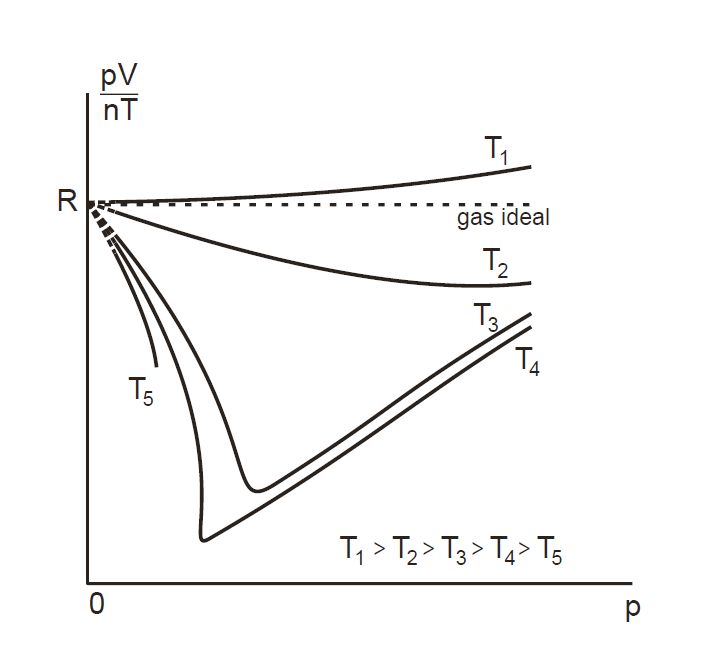
\includegraphics[scale=0.55]{diagrama-amagat.png}
\caption{diagrama de Amagat}
\end{figure}


Como podemos ver obtenemos curvas diferentes en función de la temperatura, pero si extrapolamos el comportamiento del gas a presión nula, (es imposible calcularla realmente porque presión cero es equivalente a que no haya gas), obtenemos que todas las curvas, para cualquier temperatura, conducen al mismo valor, que denotaremos como $R$.  \\

Si hacemos el mismo experimento para otro gas, las curvas serán diferentes pero análogas, y siempre que extrapolemos su comportamiento para $p=0$, obtenemos que tiene al mismo valor $R$. A este valor límite se le llama \textit{constante universal de los gases}, y que define como:

\begin{equation}
R = \lim_{p \rightarrow 0} \parentesis{\dfrac{p V}{n T}}
\end{equation}

A partir de este valor podemos definir \textbf{gas ideal} como un gas el cual verifica en todo momento que:

\begin{equation}
\dfrac{pv}{T} = R
\end{equation}

O lo que es lo mismo, que la \textbf{ecuación térmica de estado del gas ideal} es:

\begin{equation}
pV = nRT
\label{ec:1.1-006}
\end{equation}

\subsection{Ecuación energética del gas perfecto}

Trataremos ahora de determinar la forma explícita de la \textbf{ecuación energética} o \textbf{ecuación calórica} de un gas ideal. Como sabemos la energía interna puede expresarse como función de dos variables termodinámicas. En este caso escogemos $T$ y $V$. Por lo tanto:

\begin{equation}
U(T,V) \longrightarrow \D U = \pparciales{U}{T}_V \D T + \pparciales{U}{V}_T \D V = C_V \D T + \pparciales{U}{V}_T \D V
\label{ec:1.2-007}
\end{equation}

Experimentalmente hablando, la determinación del valor $\pparciales{U}{V}_T$ ha sido, y es, muy relevante, ya que puede determinar si la energía interna es independiente del volumen (entonces dicho coeficiente es nulo) o si por el contrario es dependiente. Ahora, para tratar de entender el significado físico de dicho coeficiente, vamos a reescribirlo teniendo en cuenta la siguiente relación matemática:

\begin{equation}
\pparciales{U}{V}_T \pparciales{V}{T}_U \pparciales{T}{U}_V = -1 
\end{equation}

Por lo que podemos reescribir esto como: 

\begin{eqnarray}
\pparciales{U}{V}_T & = & - \dfrac{1}{\pparciales{V}{T}_U \pparciales{T}{U}_V }  = - \pparciales{T}{V}_U \pparciales{U}{T}_V = -C_V \mu_J
\end{eqnarray}

Donde definimos como \textbf{coeficiente de Joule}:

\begin{equation}
\pparciales{T}{V}_U  = \mu_J
\end{equation} 

Entonces podemos reescribir la ecuación \ref{ec:1.2-007} como:

\begin{equation}
\D U = C_V [ \D T - \mu_j \D V]
\end{equation}

Una vez conocidos el coeficiente de Joule y la capacidad calórica podemos calcular la ecuación calórica de un gas. Para determinar cual era el valor del coeficiente de Joule (fundamental para calcular esta) tenemos que hacer evolucionar un gas en un proceso a $U=cte$. El proceso mas sencillo que mantenga la energía interna constante es aquel en el que no se intercambia calor ni trabajo con el entorno (y usando el primer principio de la termodinámica $\Delta U = 0$). \\

Ahora bien, ¿Como podemos buscar un proceso en el que ni se intercambie calor ni trabajo La expansión de un gas sin ejercer trabajo puede parecer de primeras complicada, pero dado que $W=-p \D V$, si encontramos un proceso de expansión en el con $p=0$ ya lo tenemos. Por eso Joule lo que hizo fue crear dos recipientes metálicos, unidos por un tubo ancho y corto con una válvula en el medio que los separa (e impide la mezcla). En uno de ellos había un gas, y en otro se hizo vacío. Dado que el recipiente vacío no ejerce presión sobre el otro gas, si abrimos una válvula, no se ejercerá trabajo, ya que no hay presión. Este fenómeno se conoce como \textit{expansión libre contra el vacío}. \\

Para comprobar que no se intercambiaba calor, sumergío el recipiente en agua (que se encontraba en equilibrio térmico con el gas y el recipiente antes de realizar el experimento), para ver si la temperatura de esta variaba a lo largo del experimento. Si la temperatura variaba significaba que no se intercambiaba energía térmica, y por lo tanto no se intercambiaba calor. Entonces el proceso ocurría a calor y temperatura constante.


\begin{figure}[h!] \centering
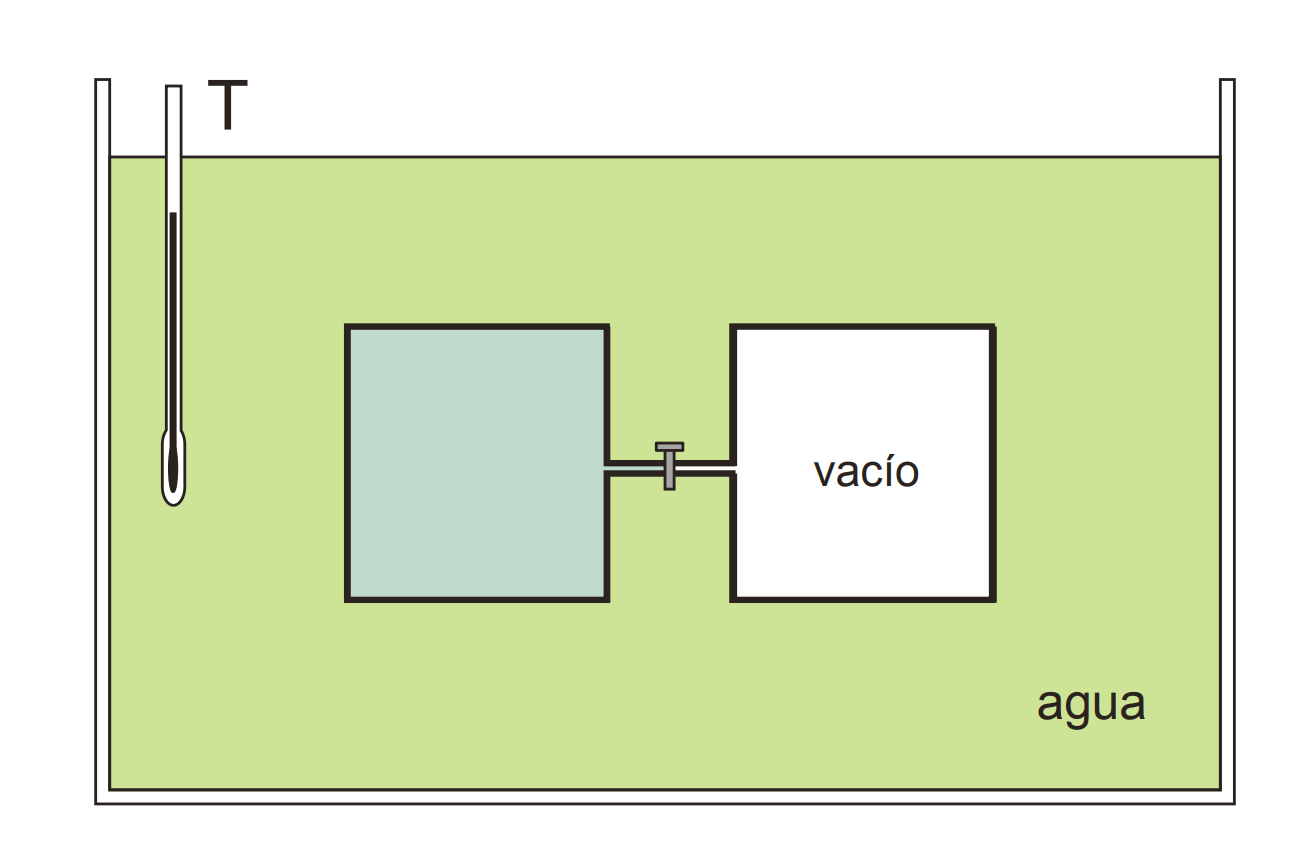
\includegraphics[scale=0.55]{experiencia-joule.png}
\caption{Experiencia de Joule}
\end{figure}

Como el volumen del gas ha variado pero no su temperatura (y la energía interna del sistema se mantuvo constante) tenemos que según la experiencia de Joule:

\begin{equation}
\mu_J = \pparciales{T}{V}_U = 0
\end{equation}

Consecuentemente hemos demostrado que la temperatura de un gas no depende del volumen, y según la siguiente relación tampoco depende de la presión:

\begin{equation}
\pparciales{U}{p}_T =  \pparciales{p}{V}_T \pparciales{V}{U}_T= 0
\end{equation}

Y por lo tanto tenemos que hemos deducido que:

\begin{equation}
U = U(T)  \Longrightarrow \D U = C_V \D T = n c_V \D T \label{ec:1.2-014} 
\end{equation}


Que es la \textit{forma diferencial de la ecuación energética} para un gas ideal. Sin embargo si estudiamos con detalle podemos ver diversos fallos en la \textit{experiencia de Joule}. Puede que tanto el termómetro usado no tuviera la suficiente precisión, y dado que la capacidad calorífica del agua es muy superiro a la del gas, para incrementar levemente la temperatura del agua debemos aportarle bastante calor. De hecho experimentos mas recientes demostraron 

\begin{equation}
\pparciales{U}{p}_T = f(T)
\end{equation}

por lo que $U = U(T,p)$, en contra de la experiencia de Joule, aunque de todos modos la variación de temperatura es muy pequeña en una \textit{expansión libre}. \\


Entonces hemos calculado tanto la ecuación térmica y energética para un gas ideal. Sin embargo esta última depende de $C_V$, que no sabemos como se comporta, aunque si estudiamos desde la mecánica estadística el comportamiento de un gas ideal monoatómico podemos llegar a la conclusión de que $C_V \neq C_V(T,p)$. Entonces podemos establecer (desde un punto de vista teórico) una nueva propiedad adicional: $C_V$ es constante. Entonces definimos como \textbf{gas perfecto} aquel que verifica \ref{ec:1.1-006} y que $C_V$ es constante. Entonces podemos deducir de \ref{ec:1.2-014} la  \textit{forma integral de la} \textbf{ecuación energética del gas perfecto}. 

\begin{equation}
\Delta U = C_V \Delta T
\end{equation}

Hay que recordar que esta expresión es válida para \textit{cualquier} proceso del gas ideal perfecto, no solo para procesos isocóricos. \\


Otra forma de justificar la forma diferencial de la ecuación energética es usar directamente la ecuación $pV=nRT$ y expresar en la \textit{ecuación energética diferencial} la entropía $S$ en función de $T$ y $V$ ($S=S(T,V)$). Sin embargo es redundante, y llegamos al a misma conclusión que en \ref{ec:1.2-014}. \\

Vamos a seguir estudiando relaciones para los gases ideales, por lo que según la ley de mayer generalizada tenemos que :

\begin{equation}
C_P - C_X = \dfrac{T \alpha^2 X}{k_T}  \Longrightarrow C_P - C_V = \dfrac{T \alpha^2 V}{k_T}
\end{equation}

Como sabemos, para un gas ideal $\alpha = 1/T$ y $k_T = 1/p$, entonces:

\begin{equation}
C_P - C_V = \dfrac{p V}{T} = nR \Longrightarrow c_p - c_v = R
\label{ec:1.2-018}
\end{equation}


Ahora vamos a aplicar esta relación para demostrar que $\D H = C_P \D T$. Tenemos que por definición:

\begin{equation}
H = U +pV = U(T) + nRT = H(T)
\end{equation}

Si diferenciamos esta expresión:

\begin{equation}
\D H = \D U + d(pV) = C_V \D T + nR \D T  = (C_V + nR) \D T = C_p \D T
\end{equation}

Entonces tenemos que la entalpía depende solo de la temperatura, calculando la ecuación energética diferencial en lenguaje entalpía válida para cualquier proceso y no solo para procesos isobáricos. \\

Ahora vamos a analizar la ecuación energética en lenguaje entrpía para un gas ideal. Para ello expresamos $S = S(p,T)$:

\begin{equation}
\D S = \pparciales{S}{p}_T \D p + \pparciales{S}{T}_p \D T =
-\pparciales{V}{T}_p \D p + \dfrac{C_p}{T} = n c_p \dfrac{\D T}{T} - nR \dfrac{\D p}{p}
\end{equation}

Donde hemos usado una ley de maxwell y que Integrando la ecuación para un gas perfecto obtenemos que:

\begin{equation}
S = n c_p \ln T - nR \ln_p + S_0
\end{equation}

\subsection{Trasformaciones adiabáticas de un gas perfecto}

Supongamos un sistema cerrado ($n$ constante) que experimenta una trasformación adiabática reversible. En esta parte vamos a deducir las expresiones para calcular como evolucionan la presión, temperatura y volumen si un gas perfecto sufre dicha trasformación. \\


 Por ser reversible $\D' Q = T \D S$, y por ser adiabática $T\D S = 0$. Entonces tenemos que la variación de energía interna del gas solo dependerá del trabajo $\D ' W = - p \D V$. También sabemos que para un gas ideal $\D U = n c_v \D T = \D ' W$. Entonces podemos escribir

\begin{equation}
- p \D V = n c_V \D T
\end{equation}

que substituyendo $p$ por la ecuación térmica (ec. \ref{ec:1.1-006}) podemos obtener que

\begin{equation}
\dfrac{nRT}{V} \D V = - n c_v  \D T \Longrightarrow \dfrac{\D V}{V} = - \dfrac{c_V}{R} \dfrac{\D T}{T}
\end{equation}

Si definimos $c_p/c_V = \gamma$, y usamos la ley de mayer (ec. \ref{ec:1.2-018}) tenemos que:

\begin{equation}
\dfrac{\D V}{V} = - \dfrac{1}{\gamma -1} \dfrac{\D T}{T}
\end{equation}

Y si es un gas perfecto tenemos que $\gamma = cte$, por lo que podemos integrar la ecuación:

\begin{equation}
\ln V - \ln V_0 = \dfrac{1}{\gamma - 1} \ccorchetes{\ln T_0 - \ln T}
\end{equation}


de lo que se puede deducir que

\begin{equation}
T^{\frac{1}{\gamma -1}} V = T_0^{\frac{1}{\gamma -1}} V_0 \Longleftrightarrow T V^{\gamma -1} = T_0 V^{\gamma-1}
\label{ec:1.3-027}
\end{equation}


Y si vamos substituyendo por la ecuación térmica de estado obtenemos las relaciones $p-V$ y $p-T$:

\begin{equation}
p V^{\gamma} = p_0 V_0^{\gamma} = \cte
\end{equation}

\begin{equation}
p^{\gamma - 1}T^{\gamma} = p_0^{\gamma -1} T^{\gamma} = \cte
\end{equation}

Ahora, una vez deducidas estas ecuaciones podemos estudiar como se comporta la \textit{fórmula de Reech} para un gas ideal. Como sabemos:

\begin{equation}
k_T = \pparciales{V}{p}_T = -  \dfrac{nRT}{p^2} = - \dfrac{V}{p}
\end{equation}

Y ahora podemos calcular $k_S$ usando las relaciones anteriores:

\begin{equation}
k_S = \pparciales{V}{p}_S = - \dfrac{ \cte}{\gamma} \dfrac{1}{p^{\gamma-1}} = - \dfrac{1}{\gamma} \dfrac{V}{p}
\end{equation}

De lo que podemos obtener que:

\begin{equation}
\dfrac{k_T}{k_S} = \gamma
\end{equation}

lo cual tiene mucho sentido ya que sabemos que 

\begin{equation}
\dfrac{k_T}{k_S} = \dfrac{C_p}{C_V}
\end{equation}

Esto también nos revela el comportamiento de las curvas adiabáticas e isotermas en un diagrama $p-V$, ya que:

\begin{equation}
\pparciales{p}{V}_S = - \gamma \dfrac{p}{V}
\end{equation}

\begin{equation}
\pparciales{p}{V}_T = - \dfrac{p}{V}
\end{equation}

Que si las representamos podemos ver que la pendiente de la curva adiabática será $\gamma$ veces mayor (en valor absoluto) que la curva isoterma. Esto implica directamente que:



Y también podemos calcular el trabajo que se realiza en un proceso adiabático, que viene dado por

\begin{equation}
W = \Delta U = n c_V \Delta T = \dfrac{p_fV_f - p_i V_i}{\gamma}
\end{equation}


\subsection{Trasformaciones politrópicas de un gas perfecto}

En primer lugar tenemos que entender que casi todas las trasformaciones con las que trabajamos ocurren dejando alguna variable constante: isotermas, isobáricas ... Ahora vamos a estudiar el caso mas general, suponiendo que una variable $a$ (puede ser cualquier cosa, entropía, entalpía...) permanece constante. Entonces si la capacidad calorífica a $a$ constante permanece constante durante el proceso, llamaremos a la trasformación una \textit{trasformación politrópica}. En general la capacidad calorífica en dicho proceso se define como:

\begin{equation}
C_a = \parentesis{\dfrac{\D ' Q}{\D T}}_a
\end{equation}

Y entonces podemos construir la siguiente relación para un gas ideal:

\begin{equation}
\D U = C_V \D T = C_a \D T - \dfrac{nRT}{V} \D V 
\end{equation}

Y separando las variables:

\begin{equation}
\dfrac{C_V - C_a}{T} \D T + \dfrac{nR}{V} \D V  = 0 \Longrightarrow  \dfrac{\D T}{T} + \dfrac{C_p - C_V}{C_V - C_a} \dfrac{\D V}{V} = 0
\end{equation}

Ahora introducimos el \textit{índice de politropía} $n$ como el cociente:

\begin{equation}
n = \dfrac{C_p - C_a}{C_V - C_a} \label{ec:1.4-040}
\end{equation}

Lo cual si restamos por uno obtenemos que:

\begin{equation}
n - 1 = \dfrac{C_p - C_a - (C_V - C_a)}{C_v - C_a} = \dfrac{C_p - C_V}{C_V - C_a}
\end{equation}

por lo que

\begin{equation}
\dfrac{\D T}{T} + (n-1) \dfrac{\D V}{V} = 0
\end{equation}


Entones podemos integrar y obtener:

\begin{eqnarray}
T V^{n-1} & = & T_0 V_0^{n-1} \\ \nonumber\\
p V^{n} & = & p_0 V_0^n \\ \nonumber\\
p^{1-n}T^n & =  & p_0^{1-n}T_0^n
\end{eqnarray}

Entonces podemos entender muchas de las trasformaciones que hemos visto entendiendo $C_a$ o $n$. Por ejemplo:

\begin{itemize}
\item \textbf{Isocórica:} en las ecuaciones isobáricas tenemos que $C_a = C_V$, de lo que podemos deducir que $n=\infty$ usando la ecuación \ref{ec:1.4-040}

\item  \textbf{Isobárica:}  tenemos que $C_a = C_p$. Igual que antes podemos deducir que $n = 0$.

\item \textbf{Isotérmica:} tenemos que en este caso $p_f V_f = p_i V_i$, esto solo puede ocurrir si $n = 1$. Para que esto ocurra $C_a = \infty$ ya que evidentemente $C_p \neq C_V$. 

\item \textbf{Adiabática reversible:} tenemos que en este caso la relación se cumple si $n = \gamma$, por lo que $C_a = 0$.  

\end{itemize}


También podemos representar las curvas en $p-V$, de lo que podemos entender una cosa: a mayor índice de politropía mayor es la pendiente de la curva. 


\subsection{Mezcla de gases perfectos} 

Ahora vamos a estudiar que ocurre con un sistema constituido por varios gases (sistemas multicomponentes) distribuidos de manera homogénea (si estudias dos porciones diferentes del volumen, no puedes diferenciar la composición). Estos gases, además, serán gases perfectos químicamente inertes entre sí. \\

Al igual que en las secciones anteriores definimos que es un gas perfecto y un gas ideal, nosotros definimos como \textbf{mezcla ideal de gases perfectos} a aquella mezcla que verifica:

\begin{equation}
p = \sum_{i=1}^N \parentesis{n_i \dfrac{RT}{V}} = n \dfrac{RT}{V}
\label{ec:1.5-046}
\end{equation}

donde $N$ es la cantidad de gases que hay, $n_i$ los moles del gas $i$, y $n$ el número de total de moles de los gases. Además se verificará que la energía interna del sistema será igual a la suma de las energías internas que tendría cada gas por separado (con la misma temperatura...):

\begin{equation}
U = \sum_{i=1}^N U_i^0 = \sum_{i=1}^N n_i u_i^0
\end{equation}

donde $u_i^0$ representa la energía interna molar. \\

Ahora vamos a estudiar uno de los hechos experimentales mas relevantes a la hora de estudiar las mezclas: cuando se determinan las presiones ejercidas por cantidades desconocidas de distintos gases, y se comparan con la presión obtenida cuando las mismas cantidades de los mismos gases se introducen todos juntos en el mismo recipiente, tenemos que la suma de todas las presiones de cada gas, y la presión total es exactamente igual. Este resultado se generaliza en la \textbf{ley de Dalton} o \textbf{ley de las presiones parciales}. \\

Se denomina \textbf{presión parcial} $p_i$, de un componente en una mezcla gaseosa a la presión que ejercería ese gas si ocupara el volumen total de la mezcla con la misma temperatura que está. La ecuación que generaliza este resultado es la ecuación \ref{ec:1.5-046}, que si lo divides entre la expresión de la presión parcial


\begin{equation}
p_i = n_i \dfrac{RT}{V}
\end{equation}

obtenemos la expresión que relaciona la presión parcial y la fracción molar ($\chi_i$): 

\begin{equation}
p_i = \dfrac{n_i}{n} p = \chi_i p
\end{equation}

El concepto de presión parcial no solo es un concepto matemático, es un concepto físico. \\

Ahora demostraremos que para una mezcla de gases ideales inertes, las funciones de estado (entropía, potenciales) son aditivos (tal y como la energía interna). Para esto vamos a emplear un recipiente conocido como el recipiente de van't Hoff que nos permite realizar la mezcla o la separación de los gases mediante un proceso reversible. \\

Supongamos dos gases ideales encerrados en un recipiente que se halla dividido por una pared C permeable para uno de los gases (gas 1), e impermeable para el otro (gas 2). El volumen a ambos lados de C es el mismo ($V$). Entonces tenemos que en uno de los lados están los dos gases, y en el otro hay vacío. Lo único que impide que de forma natural el gas 1 ocupe el espacio vacío es un pistón A, que podemos mover nosotros. En el lado opuesto, pegado a la pared, hay un pistón B solo permeable para el gas 2. Entonces comenzamos a mover ambos pistones poco a poco (infinitamente despacio) hacia el lado del vacío. El proceso será entones isotermo (ya están en equilibrio térmico) y reversible (lo hacemos infinitamente despacio), por lo que lo único que no tiene porque haber es equilibrio mecánico, pudiendo ejercer presión el gas 1 sobre el pistón B (ya que es impermeable), y no sobre A (en el otro lado hay vacío) y C (es impermeable); y el gas 2 sobre C. Sin embargo en todo momento ocurrirá una cosa, que la presión que ejerce 1 sobre B y la que ejerce 2 sobre C se anulan, por lo que realmente la fuerza total resultante sobre cualquier pistón es cero, y el trabajo realizado global es cero, ya que ni el volumen de A y B están cambiando (esto se debe a que en realidad si que hay equilibrio mecánico).  \\

Como el proceso fue isotérmico y $\D U =  n c_v  \D_T$ tenemos que la energía interna no cambió, y como no se ejerció trabajo pues $\D W = 0$. Además como fue reversible tenemos que $\D Q = T \D S$, por lo que podemos deducir que en realidad $T \Delta S = 0$, por lo la entropía inicial y final no ha variado. Podemos ver facil mente que esto implica que la entropía de la mezcla es la misma que la entropía de los dos gases por separado. Entonces si definimos como \textbf{entropía parcial} de un gas de la mezcla como la entropía que tendría dicho gas individualmente al ocupar el mismo volumen con la misma temperatura de la mezcla. Entonces el \textbf{teorema de Gibbs} nos dice que la entropía de una mezcla de gases perfectos no reaccionantes es siempre igual a la suma de las entropías parciales:

\begin{equation}
S_{\mathrm{mezcla}}= \sum_{i=1}^N S_i (T_m,V_m) 
\end{equation}

siendo $N$ el númeor de gases, $S_i$ la entropía parcial del gas $i$ y $T_m$ y $V_m$ la temperatura y volumen de la mezcla.




\end{document}

